\section{杠杆的应用}\label{sec:7-3}

从上节实验我们应该得到,杠杆的平衡条件是
$$ \textbf{动力} \times \textbf{动力臂} =  \textbf{阻力} \times \textbf{阻力臂} \; \juhao $$

用 $F_1$ 表示动力,$F_2$ 表示阻力,$l_1$ 表示动力臂,$l_2$ 表示阻力臂,上式可以写成
$$ F_1 \cdot l_1 = F_2 \cdot l_2 \;\juhao $$

把杠杆的平衡条件改写成
$$ \dfrac{\text{阻力}}{\text{动力}} = \dfrac{\text{动力臂}}{\text{阻力臂}} \qquad \text{或} \qquad \dfrac{F_2}{F_1} = \dfrac{l_1}{l_2} \;\text{,} $$

就可以看出:要使杠杆平衡,\CJKunderwave{动力臂是阻力臂的几倍,动力就是阻力的几分之一}。
例如,用杠杆撬一块重 2000 牛顿的石头,如果动力臂是 120 厘米,阻力臂是 30 厘米,
即动力臂是阻力臂的四倍,那么动力只要是阻力的四分之一,即 500 牛顿就够了。

掌握了杠杆的平衡条件,我们可以根据需要来自觉地利用杠杆。

\CJKunderwave{为了省力,我们应该用动力臂比阻力臂长的杠杆}。
撬石头的长棒和抽水机的柄都是这样的杠杆。
图 \ref{fig:7-5} 中的独轮车、钳子、起子也是这种省力的杠杆。

\begin{figure}[htbp]
    \centering
    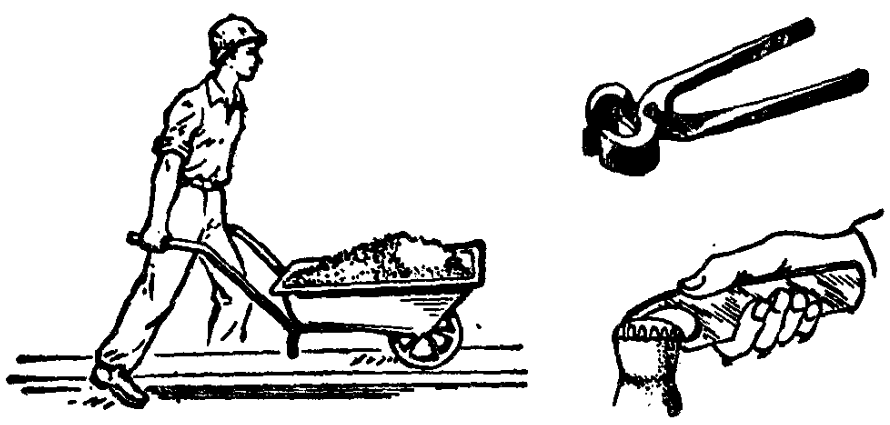
\includegraphics[width=0.7\textwidth]{../pic/czwl1-ch7-5}
    \caption{省力杠杆}\label{fig:7-5}
\end{figure}

动力臂比阻力臂短的杠杆,显然要费力,但是它会给我们带来别的好处。
我们的前臂就是这样的杠杆(图 \ref{fig:7-6})。
当曲肘将手中重物举起时,肘关节 $O$ 是支点,肌肉缩短,动力作用点 $A$ 移动不大的距离,
阻力作用点 $B$ 却移动了相当大的距离;费了力,但是省了距离。
\begin{figure}[htbp]
    \centering
    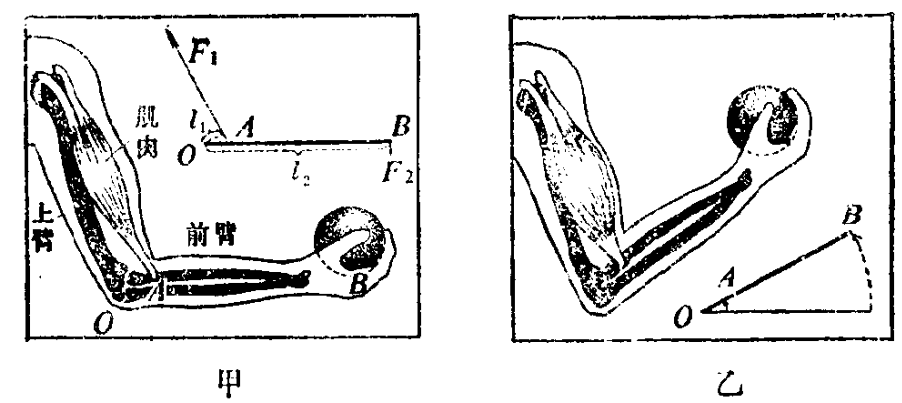
\includegraphics[width=0.8\textwidth]{../pic/czwl1-ch7-6}
    \caption{}\label{fig:7-6}
\end{figure}
可见,\CJKunderwave{为了省距离,应该用动力臂比阻力臂短的杠杆}。
图 \ref{fig:7-7} 中的钓鱼杆、剪刀、缝纫机的踏板都是这种费力但省距离的杠杆。

\begin{figure}[htbp]
    \centering
    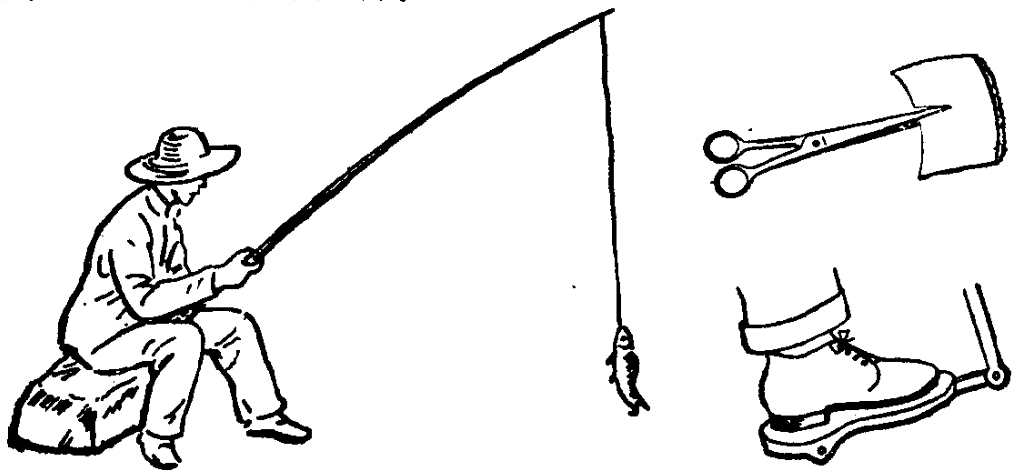
\includegraphics[width=0.7\textwidth]{../pic/czwl1-ch7-7}
    \caption{费力杠杆}\label{fig:7-7}
\end{figure}

我们使用杠杆,可以省力,但要多移动距离,也可以少移动距离,但要费力,
\CJKunderwave{又省力又少移动距离的杠杆是没有的}。

除了以上两类杠杆以外,还有一类动力臂和阻力臂相等的杠杆。
前边讲过的天平就是这样的杠杆,横梁平衡时砝码和被称物体同样重,所以它们的质量相等。

原来静止的杠杆,平衡条件一旦被破坏,杠杆就要转动。利用这个现象可以制成简单的自动机构。
锅炉的保险阀门就是这样的机构,图 \ref{fig:7-8} 是它的示意图。
当阀门 $S$ 受到的蒸汽压力超过安全值时,杠杆 $OAB$ 的平衡就被破坏,于是杠杆转动,阀门打开,
蒸汽跑掉一部分,锅炉内的蒸汽压力减小,保证了锅炉的安全。

\begin{figure}[htbp]
    \centering
    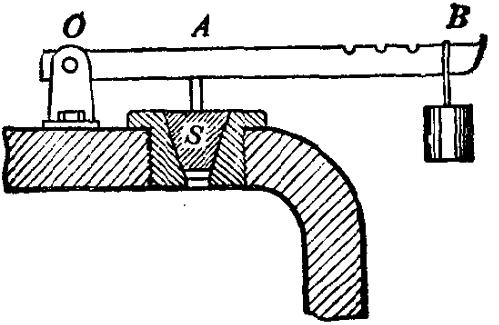
\includegraphics[width=0.4\textwidth]{../pic/czwl1-ch7-8}
    \caption{}\label{fig:7-8}
\end{figure}


\nonumsection{阅读材料:我国古代对杠杆的应用}

杠杆在我国古代就有了许巧妙的应用。大约在三千多年以前就有用来捣谷的舂(图 \ref{fig:7-9}),
用来在井上汲水的桔槔(图 \ref{fig:7-10}),还有能够做精确测量的天平和杆秤等等。

\begin{figure}[htbp]
    \centering
    \begin{minipage}{7cm}
    \centering
    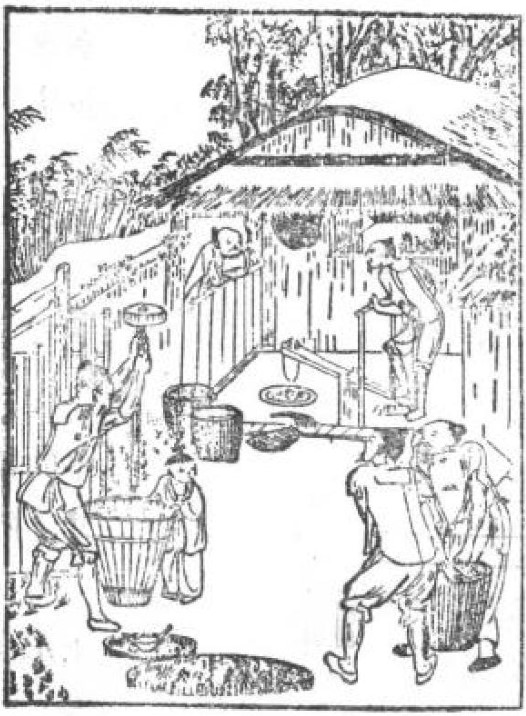
\includegraphics[width=6cm]{../pic/czwl1-ch7-9}
    \caption{舂(采自古书《天工开物》)}\label{fig:7-9}
    \end{minipage}
    \qquad
    \begin{minipage}{7cm}
    \centering
    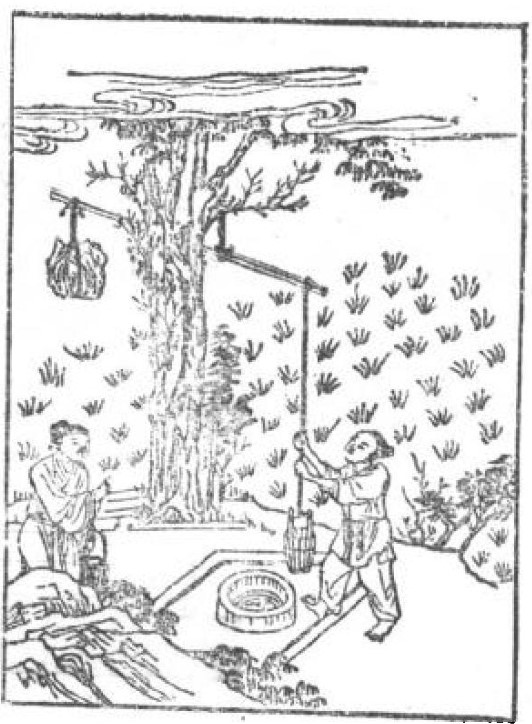
\includegraphics[width=6cm]{../pic/czwl1-ch7-10}
    \caption{桔槔}\label{fig:7-10}
    \end{minipage}
\end{figure}

\begin{figure}[htbp]
    \centering
    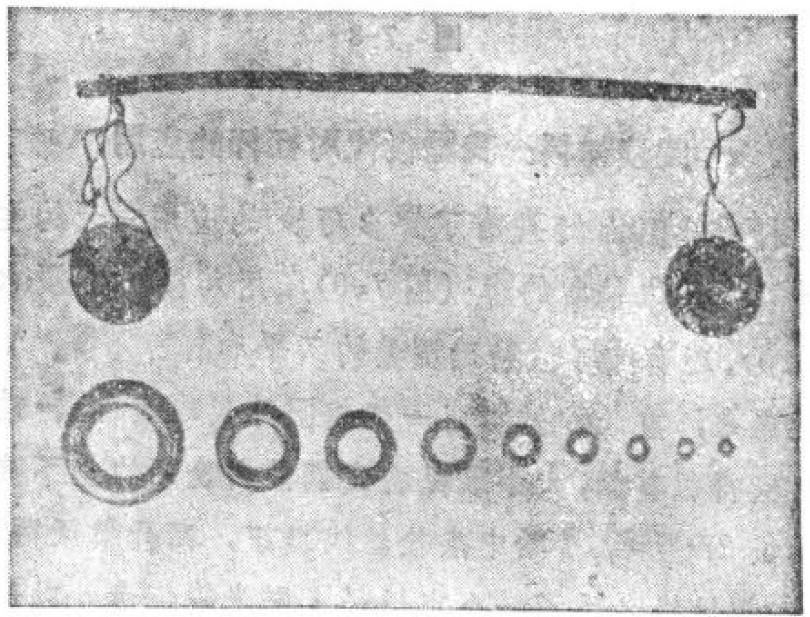
\includegraphics[width=0.6\textwidth]{../pic/czwl1-ch7-11}
    \caption{湖南长沙左家公山战国楚墓出土的天平和砝码}\label{fig:7-11}
\end{figure}


近年来,在长沙发掘出一架战国时代的天平和砝码(图 \ref{fig:7-11}),做得很精细,大小跟现在我们做实验用的差不多。
木制的横梁长 27 厘米,横梁中点拴丝线提纽,离开横梁两端各 0.7 厘米处,用丝线各系了一个直径是 4 厘米的铜盘。
砝玛共有九个,最大的是 12.5 克,最小的只有 0.6 克。从这架天平看,当时的称量的确相当精确了。

对于杠杆的原理,我们祖先也很注意研究,在公元前 4 世纪至 3 世纪成书的《墨经》中,已经有了精辟的论述。
例如谈到天平的平衡时说:“衡木:加重于其一旁,必捶——重相若也。”
意思是:天平横梁的一臂加重物,另一臂必须加砝码,两者必须等重,才能平衡。



\lianxi

(1) 参照图 \ref{fig:7-1} 、\ref{fig:7-2} 、\ref{fig:7-6},画出图 \ref{fig:7-5} 、\ref{fig:7-7} 中各物体的杠杆示意图,
并在示意图上标出支点、动力、阻力、动力臂、阻力臂。

(2) 跷跷板也是一个杠杆(图 \ref{fig:7-12}),图中的大人比小孩重,为什么却被小孩翘起?
大人怎样才能把跷跷板压下来?

\begin{figure}[htbp]
    \centering
    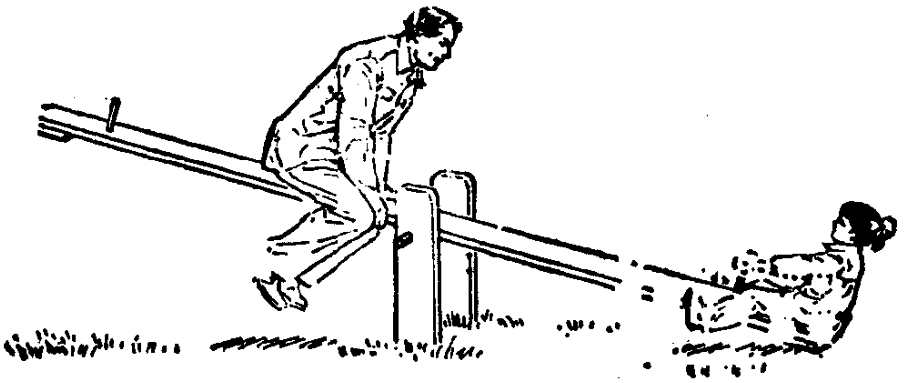
\includegraphics[width=0.7\textwidth]{../pic/czwl1-ch7-12}
    \caption{}\label{fig:7-12}
\end{figure}


(3) 除了书中有的和老师讲过的,再举出一些生活中常见的杠杆实例,并分别说明是省力、费力还是等臂的。

(4) 图 \ref{fig:7-13} 甲所示的杠杆是平衡的。如果照图乙那样在支点两侧的钩码下分别加挂一个等重的钩码,
杠杆还能平衡吗?为什么?

\begin{figure}[htbp]
    \centering
    \begin{minipage}{7cm}
    \centering
    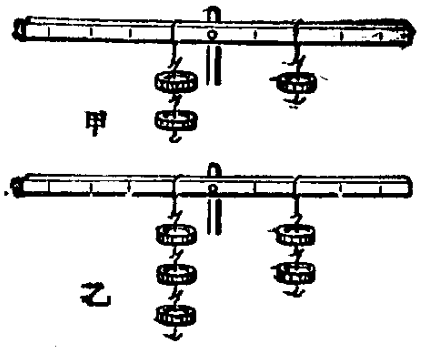
\includegraphics[width=6cm]{../pic/czwl1-ch7-13}
    \caption{}\label{fig:7-13}
    \end{minipage}
    \qquad
    \begin{minipage}{7cm}
    \centering
    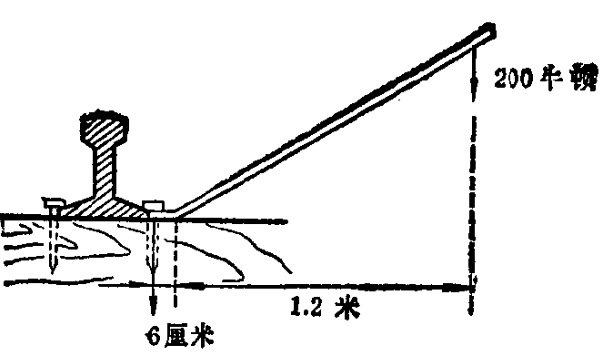
\includegraphics[width=7cm]{../pic/czwl1-ch7-14}
    \caption{}\label{fig:7-14}
    \end{minipage}
\end{figure}


(5) 用道钉撬来撬铁路枕木上的道钉(图 \ref{fig:7-14}),加在道钉撬上的力是 200 牛顿,它的力臂是 1.2 米,阻力臂是 6 厘米。
求道钉对道钉撬的阻力。

(6) 在图 \ref{fig:7-2} 中,如果加在柄上的动力 $F_1$ 是 180 牛顿,动力臂 $l_1$ 是50 厘米,
阻力臂 $l_2$ 是20 厘米。求活塞对柄的阻力 $F_2$ 是多少牛顿。

(7) 阿基米德曾经说过,给他一根足够长的杠杆,他可以把地球撬起来。他这个说法有道理吗?能够实现吗?



\nonumsection{小制作:自制天平}

把用过的圆珠笔心的头拔掉,用它的塑料管作天平的横梁(也可以用均匀的细木条来作横梁)。
在横梁的中点穿孔,拴一个提纽。在横梁的两端各穿一个孔,把两块同样的圆硬纸片作为秤盘,
分别用三条细线拴在横梁两端的孔上。拿硬币和小硬纸片当作砝码,
就可以用你自己制作的这个小天平来称量你手边的铅笔、橡皮等小物品的质量了。


